\ifx\wholebook\relax \else

\documentclass[b5paper]{article}
\usepackage[nomarginpar
  %, margin=.5in
]{geometry}

\addtolength{\oddsidemargin}{-0.05in}
\addtolength{\evensidemargin}{-0.05in}
\addtolength{\textwidth}{0.1in}

\usepackage[en]{../../../prelude}

\setcounter{page}{1}

\begin{document}

\title{Binary Search Tree}

\author{Larry~LIU~Xinyu
\thanks{{\bfseries Larry LIU Xinyu } \newline
  Email: liuxinyu95@gmail.com \newline}
  }

\maketitle
\fi

\markboth{Binary search tree}{Elementary Algorithms}

\ifx\wholebook\relax
\chapter{Binary Search Tree}
\numberwithin{Exercise}{chapter}
\fi

% ================================================================
%                 Introduction
% ================================================================
\section{Introduction}
\label{introduction} \index{binary search tree}

Array and list are typically considered the basic data structures. However, we'll see they are not necessarily easy to implement in chapter 11. Upon imperative settings, array is the most elementary data structures. It is possible to implement linked-list using arrays (section  10.3 in \cite{CLRS}). While in functional settings, linked-list acts as the building blocks to create array and other data structures.

We start from Binary Search Trees as the `hello world' data structure. Let us see an interesting programming problem given by Bentley in {\em Programming Pearls}\cite{Bentley}. It is about to count the number of words in text. Here is an example solution:\index{word counter}

\lstset{language=C++, frame=single}
\begin{lstlisting}
int main(int, char**) {
    map<string, int> dict;
    string s;
    while (cin >> s)
        ++dict[s];
    for (auto it = dict.begin(); it != dict.end(); ++it)
        cout << it->first << ": " << it->second << "\n";
}
\end{lstlisting}

We can run it to count the words in a text file:

\begin{verbatim}
$ cat bbe.txt | ./wordcount > wc.txt
\end{verbatim}

The map provided in library is a kind of balanced binary search tree. Here we use the word as the key, and its occurrence number as the value. This program runs fast, which reflects the power of binary search tree. Before dive into it, let us first see the more generic tree, the binary tree. A binary tree can be defined recursively. It is

\index{binary tree}

\begin{itemize}
\item either empty;
\item or contains 3 parts: the element, and two sub-trees called left and right children.
\end{itemize}

Figure \ref{fig:binary-tree-example} shows an example of binary tree.

\begin{figure}[htbp]
  \centering
  \subcaptionbox{Binary tree structure}{\includegraphics[scale=0.5]{img/lvr.ps}} \\
  \subcaptionbox{A binary tree}{\includegraphics[scale=0.5]{img/btexample.ps}}
  \caption{Binary tree concept and an example.}
  \label{fig:binary-tree-example}
\end{figure}

A binary search tree is a special binary tree that its elements are comparable\footnote{It is abstract ordering, not limit to magnitude, but like precedence, subset of etc. the `less than' (<) is abstract in this chapter.}, and satisfies the following constraints:

\begin{itemize}
\item For any node, all the keys in its left sub-tree are less than the key in this node;
\item the key in this node is less than any key in its right sub-tree.
\end{itemize}

Figure \ref{fig:bst-example} shows an example of binary search tree. Comparing with Figure \ref{fig:binary-tree-example}, we can see the differences in keys ordering. To highlight the elements in binary search tree is comparable, we call it as {\em key}, and name the augmented satellite data as {\em value}.

\begin{figure}[htbp]
       \begin{center}
        \includegraphics[scale=0.4]{img/bst-1.ps}
        \caption{A Binary Search Tree} \label{fig:bst-example}
       \end{center}
\end{figure}

% ================================================================
% Data layout
% ================================================================
\section{Data Layout}
\index{binary search tree!data layout}

Based on the recursive definition of binary search tree, we can design the data layout as shown in figure \ref{fig:node-layout-parent}. A node stores the key as a field, it can also store augmented data (known as satellite data). The next two fields are pointers to the left and right sub-trees. To make it easy for backtracking, it can also store a parent field pointed to its ancestor node.

\begin{figure}[htbp]
       \begin{center}
        \includegraphics[scale=0.7]{img/node-layout-parent.ps}
        \caption{Node layout with parent field.} \label{fig:node-layout-parent}
       \end{center}
\end{figure}

For illustration purpose, we'll skip the augmented data. The appendix of this chapter includes an example definition. In functional settings, it is seldom to use pointers for backtracking. Typically, there is no such need, because the algorithm is usually top-down recursive. Below is the example functional definition:

\begin{Haskell}
data Tree a = Empty
            | Node (Tree a) a (Tree a)
\end{Haskell}

% ================================================================
% Insert
% ================================================================
\section{Insertion}
\index{binary search tree!insertion}

When insert a key $k$ (or along with a value) to binary search tree $T$, we need ensure the key ordering property is always hold:

\begin{itemize}
\item If the tree is empty, construct a leaf node with key = $k$;
\item If $k$ is less than the key of root, insert it to the left sub-tree;
\item Otherwise, insert it in the right sub-tree.
\end{itemize}

There is an exceptional case that $k$ is equal to the key of root. It means $k$ already exists in the tree. We can overwrite it, or append data, or do nothing. We'll skip such case handling. This algorithm is simple and straightforward. We can define it as a recursive function:

\be
\begin{array}{rcl}
insert(\nil, k) & = & Node(\nil, k, \nil) \\
insert(Node(T_l, k, T_r), k) & = & \begin{cases}
  k < k': & Node(insert(T_l, k), k', T_r) \\
  otherwise: & Node(T_l, k', insert(T_r, k)) \\
  \end{cases}
\end{array}
\ee

For the none empty node, $T_l$ denotes the left sub-tree, $T_r$ denotes the right sub-tree, and $k'$ is the key. The function $Node(l, k, r)$ creates a node from two sub-trees and a key. $\nil$ means empty (also known as NIL. This symbol was invented by mathematician André Weil for null set. It came from the Norwegian alphabet). Below is the corresponding example program in Haskell for insertion.

\begin{Haskell}
insert Empty k = Node Empty k Empty
insert (Node l x r) k | k < x = Node (insert l k) x r
                      | otherwise = Node l x (insert r k)
\end{Haskell}

This example program utilizes the {\em pattern matching} features. The appendix of this chapter provides another example without using this feature. Insertion can also be implemented without recursion. Here is a pure iterative algorithm:

\begin{algorithmic}[1]
\Function{Insert}{$T, k$}
  \State $root \gets T$
  \State $x \gets$ \Call{Create-Leaf}{$k$}
  \State $parent \gets$ NIL
  \While{$T \neq$ NIL}
    \State $parent \gets T$
    \If{$k <$ \Call{Key}{$T$}}
      \State $T \gets $ \Call{Left}{$T$}
    \Else
      \State $T \gets $ \Call{Right}{$T$}
    \EndIf
  \EndWhile
  \State \Call{Parent}{$x$} $\gets parent$
  \If{$parent = $ NIL} \Comment{tree $T$ is empty}
    \State \Return $x$
  \ElsIf{$k <$ \Call{Key}{$parent$}}
    \State \Call{Left}{$parent$} $\gets x$
  \Else
    \State \Call{Right}{$parent$} $\gets x$
  \EndIf
  \State \Return $root$
\EndFunction
\Statex
\Function{Create-Leaf}{k}
  \State $x \gets $ \Call{Empty-Node}{}
  \State \Call{Key}{$x$} $ \gets k$
  \State \Call{Left}{$x$} $ \gets $ NIL
  \State \Call{Right}{$x$} $ \gets $ NIL
  \State \Call{Parent}{$x$} $ \gets $ NIL
  \State \Return $x$
\EndFunction
\end{algorithmic}

While a bit more complex than the functional one, the iterative implementation runs faster, and it is capable to process very deep tree.

\section{Traverse}
\index{binary search tree!traverse}

Traverse is to visit every element one by one. There are 3 different ways to walk through a binary tree: (1) pre-order tree walk, (2) in-order tree walk, (3) and post-order tree walk. They are named to highlight the order of visiting key before/after sub-trees.

\begin{itemize}
\item pre-order: \textbf{key} - left - right;
\item in-order: left - \textbf{key} - right;
\item post-order: left - right - \textbf{key}.
\end{itemize}

\index{pre-order traverse} \index{in-order traverse} \index{post-order traverse}

Each `visit' operation is recursive, for example in pre-order traverse, when visit the left sub-tree, we recursively traverse it if it is not empty. For the tree shown in figure \ref{fig:bst-example}, the corresponding visiting orders are as below:

\begin{itemize}
\item pre-order: 4, 3, 1, 2, 8, 7, 16, 10, 9, 14
\item in-order: 1, 2, 3, 4, 7, 8, 9, 10, 14, 16
\item post-order: 2, 1, 3, 7, 9, 14, 10, 16, 8, 4
\end{itemize}

It is not by accident that the in-order traverse lists the elements one by one increasingly. The definition of the binary search tree ensures it is always true. We leave the proof as an exercise. Specifically, the in-order traverse algorithm is defined as:

\begin{itemize}
\item If the tree is empty, stop and return;
\item Otherwise, in-order traverse the left sub-tree; then visit the key; finally in-order traverse the right sub-tree.
\end{itemize}

We can further define a generic $map$ to apply any given function $f$ to every element in the tree along the in-order traverse. The result is a new tree mapped by $f$.

\be
\begin{array}{rcl}
map(f, \nil) & = & \nil \\
map(f, Node(T_l, k, T_r)) & = & Node(map(f, T_l), f(k), map(f, T_r))
\end{array}
\ee

If we only need manipulate keys but not to transform the tree, we can implement this algorithm imperatively.

\begin{algorithmic}[1]
\Function{In-Order-Traverse}{$T, f$}
  \If{$T \neq$ NIL}
    \State \textproc{In-Order-Traverse}(\Call{Left}{$T, f$})
    \State $f$(\Call{Key}{$T$})
    \State \textproc{In-Order-Traverse}(\Call{Right}{$T, f$})
  \EndIf
\EndFunction
\end{algorithmic}

Leverage in-order traverse, we can change the $map$ function to convert a binary search tree to a sorted list. Instead building the tree in recursive case, we concatenate the result to a list:

\be
\begin{array}{rcl}
toList(\nil) & = & [\ ] \\
toList(Node(T_l, k, T_r)) & = & toList(T_l) \doubleplus [ k ] \doubleplus toList(T_r) \\
\end{array}
\ee

We can develop a method to sort a list of elements: first build a binary search tree from the list, then turn it back to list through in-order traversing. This method is called as `tree sort'. For a given list $X = [x_1, x_2, x_3, ..., x_n]$.

\be
  sort(X) = toList(fromList(X))
\ee

And we can write it in point-free form\cite{func-composition}.

\[
  sort = toList \circ fromList
\]

Where function $fromList$ repeatedly inserts elements from a list to a tree. It can be defined to recursively process the list.

\[
\begin{array}{rcl}
fromList([\ ]) & = & \nil \\
fromList(X) & = & insert(fromList(X'), x_1) \\
\end{array}
\]

When the list is empty, the result is an empty tree; otherwise, it inserts the first element $x_1$ to the tree, then recursively inserts the rests $X' = [x_2, x_3, ..., x_n]$. By using list folding\cite{wiki-fold} (see appendix A.6), we can also define $fromList$ as the following:

\be
  fromList(X)= \fold_l(insert, \nil, X)
\ee

We can also rewrite it in Curried form\cite{curry} (also known as partial application) such as to omit parameter $X$:

\[
  fromList = \fold_l\ insert\ \nil
\]

\begin{Exercise}
\Question{Given the in-order and pre-order traverse results, re-construct the tree, and output the post-order traverse result. For example:

\begin{itemize}
\item Pre-order: 1, 2, 4, 3, 5, 6;
\item In-order: 4, 2, 1, 5, 3, 6;
\item Post-order: ?
\end{itemize}
\index{tree reconstruction}
}

\Question{Write a program to re-construct the binary tree from the pre-order and in-order traverse lists.}

\Question{For binary search tree, prove that the in-order traverse always visits elements in increase order}

\Question{Consider the performance of tree sort algorithm, what is its complexity for $n$ elements?}
\end{Exercise}

% ================================================================
% Query
% ================================================================
\section{Query}
\index{binary search tree!search}
\index{binary search tree!looking up}

Because the elements stored in binary search tree is well ordered and organized recursively. It supports varies of search effectively. This is one of the reasons people name it as binary search tree. There are mainly three types of querying: (1) look up a key; (2) find the minimum or maximum element; (3) given any node, find its predecessor or successor.

\subsection{Look up}
Because binary search tree is recursive and all elements satisfy the ordering property, we can look up a key $k$ top-down from the root as the following:

\begin{itemize}
\item If the tree is empty, terminate. The key does not exist;
\item Compare $k$ with the key of root, if equal, we are done. The key is stored in the root;
\item If $k$ is less than the key of root, then recursively look up the left sub-tree;
\item Otherwise, look up the right sub-tree.
\end{itemize}

We can define the recursive $lookup$ function for this algorithm as below.

\be
\begin{array}{rcl}
lookup(\nil, x) & = & \nil \\
lookup(Node(T_l, k, T_r), x) & = & \begin{cases}
  k = x: & T \\
  x < k: & lookup(T_l, x) \\
  otherwise: & lookup(T_r, x) \\
  \end{cases}
\end{array}
\ee

This function returns the tree node being located or empty if not found. One may instead return the value that bound to the key. However, in search implementation, we need consider using $Maybe$ type (also known as \texttt{Optional<T>}) to handle the not found case, for example:

\begin{Haskell}
lookup Empty _ = Nothing
lookup t@(Node l k r) x | k == x = Just k
                        | x < k = lookup l x
                        | otherwise = lookup r x
\end{Haskell}

If the binary search tree is well balanced, which means almost all branch nodes have both none empty sub-trees except for leaves. This is not the formal definition of balance. We'll define it in chapter 3. For a balanced tree of $n$ elements, the algorithm takes $O(\lg n)$ time to look up a key. If the tree is poor balanced, the worst case is bound to $O(n)$ time. If denote the height of the tree as $h$, we can represent the performance of look up as $O(h)$.

We can also implement looking up purely iterative without recursion:

\begin{algorithmic}[1]
\Function{Search}{$T, x$}
  \While{$T \neq $ NIL and \Call{Key}{$T$} $ \neq x$}
    \If{$x <$ \Call{Key}{$T$}}
      \State $T \gets $ \Call{Left}{$T$}
    \Else
      \State $T \gets $ \Call{Right}{$T$}
    \EndIf
  \EndWhile
  \State \Return $T$
\EndFunction
\end{algorithmic}

\subsection{Minimum and maximum}
\index{binary search tree!min/max}

From the definition, we know that less keys are always on the left. To locate the minimum element, we can keep traversing along the left sub-trees till reach to a node, where its left sub-tree is empty. In a symmetric way, keep traversing along the right sub-trees gives the maximum.

\be
\begin{array}{rcl}
min(Node(\nil, k, T_r)) & = & k \\
min(Node(T_l, k, T_r)) & = & min(T_l) \\
\end{array}
\ee

\be
\begin{array}{rcl}
max(Node(T_l, k, \nil)) & = & k \\
max(Node(T_l, k, T_r)) & = & max(T_r) \\
\end{array}
\ee

Both functions are bound to $O(h)$ time, where $h$ is the height of the tree.

\subsection{Successor and predecessor}
\index{binary search tree!succ/pred}

When treat binary search tree as a generic container (a collection of elements), it is common to traverse it with a bi-directional iterator. Start from the minimum element, one can keep moving forward with the iterator towards the maximum, or go back and forth. Below example program prints elements in sorted order.

\lstset{language=Bourbaki}
\begin{lstlisting}
void printTree (Node<T> t) {
    for (var it = Iterator(t), it.hasNext(); it = it.next()) {
        print(it.get(), ", ");
    }
}
\end{lstlisting}

Such use cases demand us to design algorithm to find the successor or predecessor of any node. The successor of element $x$ is defined as the smallest element $y$ that satisfies $x < y$. If the node of $x$ has none empty right sub-tree, then minimum element of the right sub-tree is the successor. As shown in figure \ref{fig:bst-succ}, to find the successor of 8, we search the minimum element in its right sub-tree, which is 9. If the right sub-tree of node $x$ is empty, we need back-track along the parent field till the closest ancestor whose left sub-tree is also an ancestor of $x$. In figure \ref{fig:bst-succ}, since node 2 does not have right sub-tree, we go up to its parent of node 1. However, node 1 does not have left sub-tree, we need go up again, hence reach to node 3. As the left sub-tree of node 3 is also an ancestor of node 2, node 3 is the successor of node 2.

\begin{figure}[htbp]
  \centering
  \includegraphics[scale=0.45]{img/bst-1.ps}
  \caption{The successor of 8, is the minimum one in its right sub-tree, 9; In order to find the successor of 2, we go up to its parent 1, then 3. } \label{fig:bst-succ}
\end{figure}

If we finally reach to the root when back-track along the parent, but still can not find an ancestor on the right, then the node does not have a successor. Below algorithm finds the successor of a given node $x$:

\begin{algorithmic}[1]
\Function{Succ}{$x$}
  \If{\Call{Right}{$x$} $\neq $ NIL}
    \State \Return \textproc{Min}(\Call{Right}{$x$})
  \Else
    \State $p \gets $ \Call{Parent}{$x$}
    \While{$p \neq $ NIL and $x =$ \Call{Right}{$p$}}
      \State $x \gets p$
      \State $p \gets $ \Call{Parent}{$p$}
    \EndWhile
    \State \Return $p$
  \EndIf
\EndFunction
\end{algorithmic}

This algorithm returns NIL when $x$ does not has successor. The predecessor finding algorithm is symmetric:

\begin{algorithmic}[1]
\Function{Pred}{$x$}
  \If{\Call{Left}{$x$} $\neq $ NIL}
    \State \Return \textproc{Max}(\Call{Left}{$x$})
  \Else
    \State $p \gets $ \Call{Parent}{$x$}
    \While{$p \neq $ NIL and $x =$ \Call{Left}{$p$}}
      \State $x \gets p$
      \State $p \gets $ \Call{Parent}{$p$}
    \EndWhile
    \State \Return $p$
  \EndIf
\EndFunction
\end{algorithmic}

It seems hard to find the purely functional solution, because there is no pointer like field linking to the parent node\footnote{There is \texttt{ref} in ML and OCaml, we limit to the purely functional settings.}. One solution is to left `breadcrumbs' when we visit the tree, and use these information to back-track or even re-construct the whole tree. Such data structure, that contains both the tree and `breadcrumbs' is called zipper\cite{zipper-hbook}.

Our original purpose to develop $succ$ and $pred$ functions is `to traverse all the elements' as a generic container. However, in functional settings, we typically traverse the tree in-order through $map$. We'll meet similar situations in the rest of this book. A problems valid in imperative settings may not be necessarily meaningful in functional settings. For example, to delete an element from red-black tree\cite{okasaki-blog}.

\begin{Exercise}

\Question{Use \textproc{Pred} and \textproc{Succ} to write an iterator to traverse the binary search tree as a generic container. What's the time complexity to traverse a tree of $n$ elements?}

\Question{One can traverse elements inside a range $[a, b]$ for example:

\texttt{for\_each (m.lower\_bound(12), m.upper\_bound(26), f);}

Write an equivalent functional program for binary search tree\index{range traverse}.}
\end{Exercise}

% ================================================================
%                 Deletion
% ================================================================
\section{Deletion}
\index{binary search tree!delete}
We need special consideration when delete an element from the binary search tree. This is because we must keep the ordering property, that for any node, all keys in left sub-tree are less than the key of this node, and they are all less than any keys in right sub tree. Blindly deleting a node may break this constraint.

To delete a node $x$ from a binary search tree\cite{sgi-stl}.
\begin{itemize}
\item If $x$ has no sub-trees (a leaf) or only one sub-tree, splice $x$ out;
\item Otherwise ($x$ has two sub-trees), use the minimum element $y$ of its right sub-tree to replace $x$, and splice the original $y$ out.
\end{itemize}

The simplicity comes from the fact that, for the node to be deleted, if the right sub-tree is not empty, then the minimum element is some node in it. It can't have two none empty children, and end up in the trivial case. Therefore, the node can be directly splice out from the tree.

Figure \ref{fig:del-leaf}, \ref{fig:del-1child}, and \ref{fig:del-branch} illustrate different cases for deletion.

\begin{figure}[htbp]
  \centering
  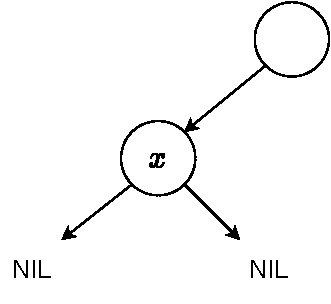
\includegraphics[scale=0.5]{img/del-leaf.ps}
  \caption{$x$ can be spliced out.} \label{fig:del-leaf}
\end{figure}

\begin{figure}[htbp]
  \centering
  \subcaptionbox{Before delete $x$.}{\includegraphics[scale=0.5]{img/del-lc-before.ps}}
  \subcaptionbox{After delete $x$, $x$ is spliced out, and replaced by its left child.}{\includegraphics[scale=0.5]{img/del-lc-after.ps}} \\
  \subcaptionbox{Before delete $x$.}{\includegraphics[scale=0.5]{img/del-rc-before.ps}}
  \subcaptionbox{After delete $x$, $x$ is spliced out, and replaced by its right sub-tree.}{\includegraphics[scale=0.5]{img/del-rc-after.ps}}
  \caption{Delete a node with only one none empty sub-tree.}
  \label{fig:del-1child}
\end{figure}

\begin{figure}[htbp]
  \centering
  \subcaptionbox{Before delete $x$.}{\includegraphics[scale=0.5]{img/del-branch-before.ps}}
  \subcaptionbox{After delete $x$, $x$ is replaced by splicing the minimum element from its right sub-tree.}{ \includegraphics[scale=0.5]{img/del-branch-after.ps}}
  \caption{Delete a node with two none empty sub-trees.}
  \label{fig:del-branch}
\end{figure}

Based on this idea, we can define the $delete$ algorithm as below:

\be
\begin{array}{rcl}
delete(\nil, x) & = & \nil\\
delete(Node(T_l, k, T_r), x) & = & \begin{cases}
  x < k: & Node(delete(T_l, x), k, T_r) \\
  x > k: & Node(T_l, k, delete(T_r, x)) \\
  x = k: & del(T_l, T_r) \\
\end{cases}
\end{array}
\ee

Function $del$ performs slicing, and mutually call $delete$ recursively to cut off the minimum from the right sub-tree.

\be
\begin{array}{rcl}
del(\nil, T_r) & = & T_r \\
del(T_l, \nil) & = & T_l \\
del(T_l, T_r) & = & Node(T_l, y, delete(T_r, y)) \\
\end{array}
\ee

Where $y = min(T_r)$ is the minimum element in the right sub-tree. Here is the corresponding example program:

\begin{Haskell}
delete Empty _ = Empty
delete (Node l k r) x | x < k = Node (delete l x) k r
                      | x > k = Node l k (delete r x)
                      | otherwise = del l r
  where
    del Empty r = r
    del l Empty = l
    del l r = let k' = min r in Node l k' (delete r k')
\end{Haskell}

This algorithm firstly looks up the node to be deleted, then executes the deletion. It takes $O(h)$ time where $h$ is the height of the tree.

The imperative deletion algorithm needs set the parent properly in addition. The following one returns the root of the result tree.

\begin{algorithmic}[1]
\Function{Delete}{$T, x$}
  \State $r \gets T$
  \State $x' \gets x$ \Comment{save $x$}
  \State $p \gets $ \Call{Parent}{$x$}
  \If{\Call{Left}{$x$} $= $ NIL}
    \State $x \gets $ \Call{Right}{$x$}
  \ElsIf{\Call{Right}{$x$} $= $ NIL}
    \State $x \gets $ \Call{Left}{$x$}
  \Else
    \Comment{neither children is empty}
    \State  $y \gets $ \textproc{Min}(\Call{Right}{$x$})
    \State \Call{Key}{$x$} $\gets$ \Call{Key}{$y$}
    \State Copy other satellite data from $y$ to $x$
    \If{\Call{Parent}{$y$} $\neq x$}
      \Comment{$y$ does not have left sub-tree}
      \State \textproc{Left}(\Call{Parent}{$y$}) $\gets$ \Call{Right}{$y$}
    \Else
      \Comment{$y$ is the root of the right sub-tree}
      \State \Call{Right}{$x$} $\gets$ \Call{Right}{$y$}
    \EndIf
    \If{\Call{Right}{$y$} $\neq $ NIL}
      \State \textproc{Parent}(\Call{Right}{$y$}) $\gets$ \Call{Parent}{$y$}
    \EndIf
    \State Remove $y$
    \State \Return $r$
  \EndIf
  \If{$x \neq $ NIL}
    \State \Call{Parent}{$x$} $\gets p$
  \EndIf
  \If{$p = $ NIL}
    \Comment{remove the root}
    \State $r \gets x$
  \Else
    \If{\Call{Left}{$p$} $= x'$}
      \State \Call{Left}{$p$} $\gets x$
    \Else
      \State \Call{Right}{$p$} $\gets x$
    \EndIf
  \EndIf
  \State Remove $x'$
  \State \Return $r$
\EndFunction
\end{algorithmic}

We assume the node to be deleted is not empty. This algorithm first records the root, creates copy reference to $x$, and its parent. If either sub-tree is empty, then we splice $x$ out. Otherwise, the node has two none empty sub-trees. We first located the minimum node $y$ in its right sub-tree, then replace the key of $x$ with the one in $y$, copy the satellite data, and finally, splice $y$ out. We also need handle the special case, that $y$ is the root of the right sub-tree.

At last, we need reset the stored parent if $x$ has only one none empty sub-tree. If the parent pointer we copied is empty, it means that we are deleting the root. In this case, we need return the new root. After the parent is set properly, we can safely remove $x$. The deletion algorithm is bound to $O(h)$ time, where $h$ is the height of the tree.

\begin{Exercise}

\Question{There is a symmetric deletion algorithm. When neither sub-tree is empty, we can replace the key by splicing the maximum node off the left sub-tree. Write a program to implement this solution.}

\end{Exercise}

\section{Random build}
\index{binary search tree!random build}
All binary search tree algorithms we give so far are bound bound to $O(h)$ time. The height $h$ of the tree impacts the performance. For a poor unbalanced tree, $O(h)$ tends to be $O(n)$. It leads to the worst case. While for well balanced tree, $O(h)$ close to $O(\lg n)$. We can gain good performance.

We'll see two well designed solutions to keep the tree balanced in chapter 3 and 4. There exists a simple method, to build the binary search tree randomly\cite{CLRS}. It decreases the possibility of giving a unbalanced binary tree. The idea is to randomly shuffle the elements before building the tree.

\begin{Exercise}
\Question{Write a randomly building algorithm for binary search tree.}
\end{Exercise}

\section{Appendix: Example programs}

Definition of binary search tree node with parent field.

\lstset{language=Bourbaki, frame=single}
\begin{lstlisting}
data Node<T> {
    T key
    Node<T> left
    Node<T> right
    Node<T> parent

    Node(T x) { key = x }
    Node(Node<T> l, T k, Node<T> r) {
        left = l, key = k, right = r
    }
}
\end{lstlisting}

Example program of insertion. It does not use pattern matching.

\begin{lstlisting}
Node<T> insert (Node<T> t, T x) {
    if (t == null) {
        return Node(null, x, null)
    } else if (t.key < x) {
        return Node(insert(t.left, x), t.key, t.right)
    } else {
        return Node(t.left, t.key, insert(t.right, x))
    }
}
\end{lstlisting}

Example program to look up a key. Purely iterative without recursion.

\begin{lstlisting}
Optional<Node<T>> lookup (Node<T> t, T x) {
    while (t != null and t.key != x) {
        if (x < t.key) {
            t = t.left
        } else {
            t = t.right
        }
    }
    return Optional(t);
}
\end{lstlisting}

Example iterative program to find the minimum of a tree.

\begin{lstlisting}
Optional<Node<T>> min (Node<T> t) {
    while (t != null and t.left != null) {
        t = t.left
    }
    return Optional(t);
}
\end{lstlisting}

Example program to find the successor of a node.
\begin{lstlisting}
Optional<Node<T>> succ (Node<T> x) {
    if (x == null) {
        return Optional.None
    } else if (x.right != null) {
        return min(x.right)
    } else {
        p = x.parent
        while (p != null and x == p.right) {
            x = p
            p = p.parent
        }
        return Optional(p);
    }
}
\end{lstlisting}

Example program to delete a node imperatively from the tree.

\begin{lstlisting}
Node<T> delete(Node<T> t, Node<T> x) {
    if (x == null) {
        return t
    }
    root, x0, parent = t, x, x.parent
    if (x.left == null) {
        x = x.right
    } else if (x.right == null) {
        x = x.left
    } else {
        y = min(x.right)
        x.key = y.key
        if (y.parent != x) {
            y.parent.left = y.right
        } else {
            x.right = y.right
        }
        if (y.right != null) {
            y.right.parent = y.parent
        }
        return root
    if (x != null) {
        x.parent = parent
    }
    if (parent == null) {
        root = x
    } else {
        if (parent.left == x0) {
            parent.left = x
        } else {
            parent.right = x
        }
    return root
}
\end{lstlisting}

\begin{thebibliography}{99}

\bibitem{CLRS}
Thomas H. Cormen, Charles E. Leiserson, Ronald L. Rivest and Clifford Stein.
``Introduction to Algorithms, Second Edition''. ISBN:0262032937. The MIT Press. 2001

\bibitem{Bentley}
Jon Bentley. ``Programming Pearls(2nd Edition)''. Addison-Wesley Professional; 2 edition (October 7, 1999). ISBN-13: 978-0201657883

\bibitem{okasaki-blog}
Chris Okasaki. ``Ten Years of Purely Functional Data Structures''. http://okasaki.blogspot.com/2008/02/ten-years-of-purely-functional-data.html

\bibitem{sgi-stl}
SGI. ``Standard Template Library Programmer's Guide''. http://www.sgi.com/tech/stl/

\bibitem{literal-program}
http://en.literateprograms.org/Category:Binary\_search\_tree

\bibitem{wiki-fold}
http://en.wikipedia.org/wiki/Foldl

\bibitem{func-composition}
http://en.wikipedia.org/wiki/Function\_composition

\bibitem{curry}
http://en.wikipedia.org/wiki/Partial\_application

\bibitem{zipper-hbook}
Miran Lipovaca. ``Learn You a Haskell for Great Good! A Beginner's Guide''. the last chapter. No Starch Press; 1 edition April 2011, 400 pp. ISBN: 978-1-59327-283-8

\end{thebibliography}

\ifx\wholebook\relax\else
\end{document}
\fi
